\documentclass[11pt]{beamer}
\usepackage{url}
\usepackage{listings}
\usetheme{CambridgeUS}

\setbeamertemplate{navigation symbols}{}
\setbeamertemplate{itemize items}[default]
\setbeamercolor{local structure}{fg=red}

\title[open-mosaic]{\textbf{open-mosaic} \\ OpenCV based mosaic generator \\ implemented in python}

\subtitle{Information Retrieval - SS 2015}

\author[Peter Spiess-Knafl]{Peter Spiess-Knafl\\ \emph{dev@spiessknafl.at}}
\date{}
\begin{document}

\maketitle

\begin{frame}
\frametitle{Motivation}
\begin{itemize}
	\item Implement a mosaic stitcher
	\item Try various feature extractions
	\item Allow for quick exchange of feature vectors
	\item Use OpenCV for Speed-Up
\end{itemize}
\end{frame}

\begin{frame}[t]
\frametitle{Mosaic}
\begin{itemize}
	\item Picture of pictures
	\item Replace areas from original picture with individual pictures
	\item Choose from a set of given images based on their colors
\end{itemize}

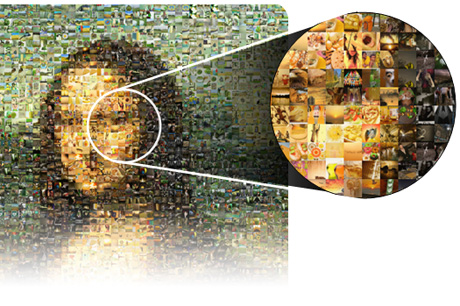
\includegraphics[width=\textwidth]{photo_mosaic.jpg}


\end{frame}

\begin{frame}
\frametitle{Approach}
\textbf{2 stages}
\begin{itemize}
	\item I: Indexing, extract features from image data set.
	\item II: Stitching, find best match and replace it.
\end{itemize}

\textbf{Index}
\begin{itemize}
	\item Extract Average H,S,V,R,G,B values for each image
	\item Scale down to 100x100 pixels
	\item Use open-cv histogram functions to extract average colors
	\item \texttt{\{"r": 118, "b": 229, "g":220, "h": 34, "s": 73, "v": 34, "file": "img\_234234.jpg" \}}
\end{itemize}
\end{frame}

\begin{frame}
\frametitle{Approach}
\textbf{Feature vector}
\begin{itemize}
	\item Average color, based on weighted channel histogram
	\item Normalized to number of pixels
\end{itemize}
\textbf{Distance vector}
\begin{itemize}
	\item Eucledian distance
	\item $\sqrt{\sum_{i=1}^n (q_i-p_i)^2}$
\end{itemize}
\end{frame}

\begin{frame}
\frametitle{Evaluation}
\textbf{Indexing:}
\begin{itemize}
	\item INRIA Holidays dataset\footnote{\url{http://lear.inrialpes.fr/~jegou/data.php}}
	\item 2.7 GB of JPEG images
	\item indexed $< 40 sec$
\end{itemize}
\textbf{Stitching}
\begin{itemize}
	\item 50 tiles / second
	\item Rather slow, due to python environment
	\item Parallelization is possible (split rows)
	\item Evaluated RGB vs. HSV
\end{itemize}
\end{frame}

\begin{frame}
\frametitle{Results}
\textbf{Input}\\

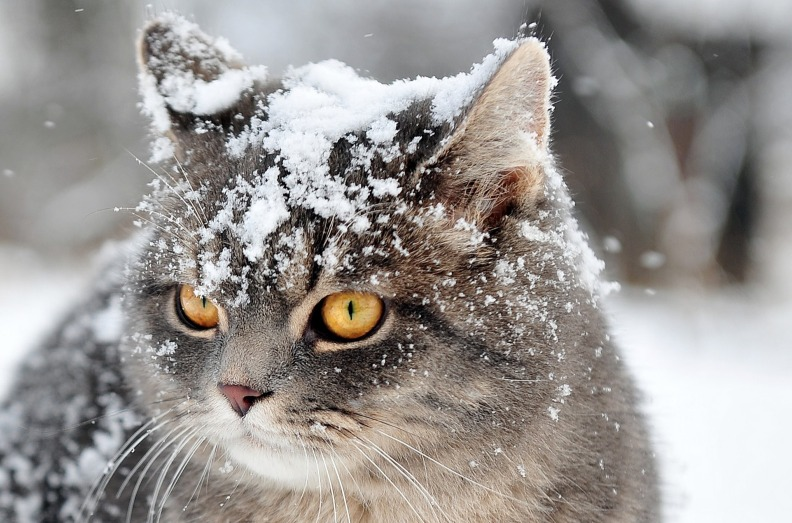
\includegraphics[width=.3\textwidth]{cat.jpg}

\textbf{RGB}\\

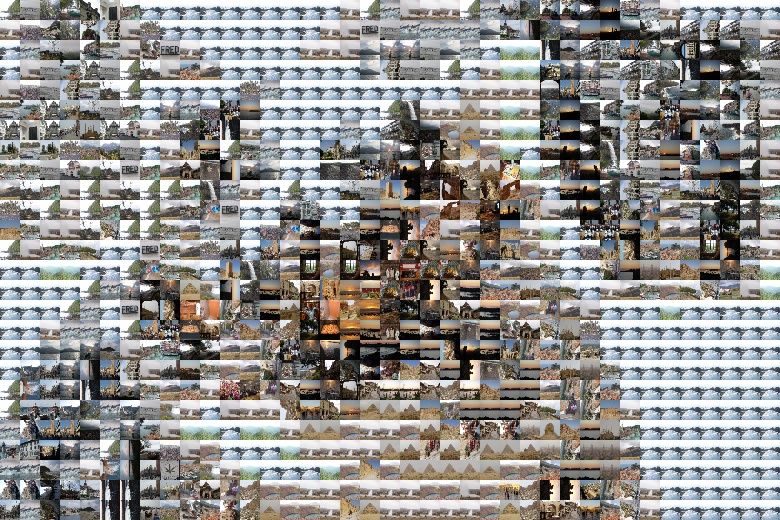
\includegraphics[width=.35\textwidth]{cat-rgb-20.jpg}
%
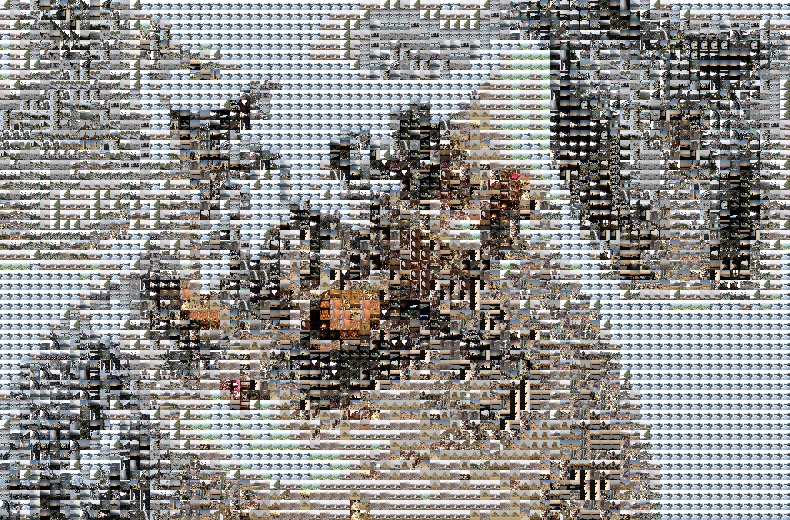
\includegraphics[width=.35\textwidth]{cat-rgb-10.jpg}
%
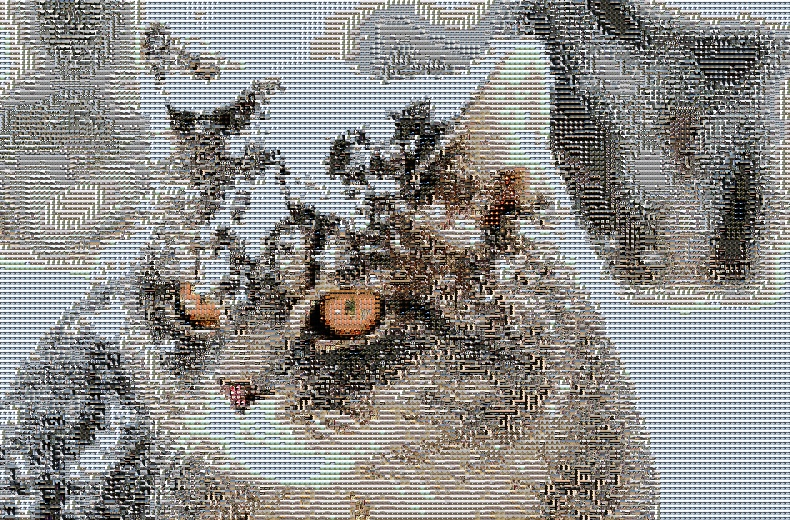
\includegraphics[width=.35\textwidth]{cat-rgb-5.jpg}
\end{frame}

\begin{frame}
\frametitle{Results}
\textbf{RGB}\\

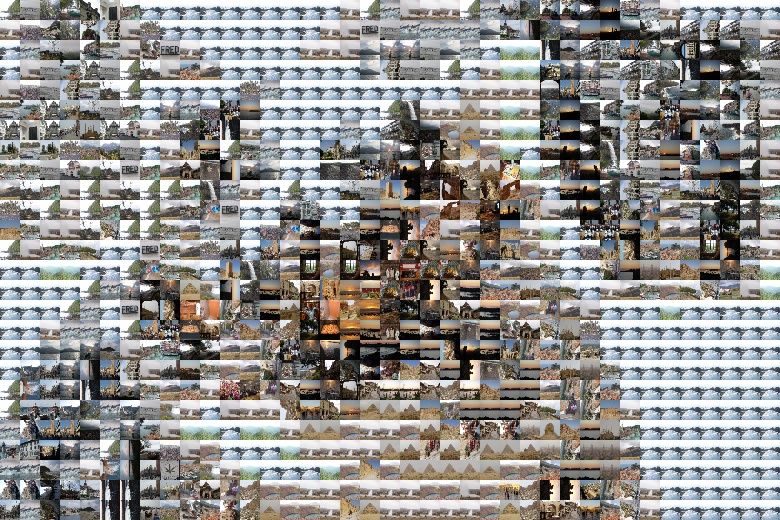
\includegraphics[width=.35\textwidth]{cat-rgb-20.jpg}
%
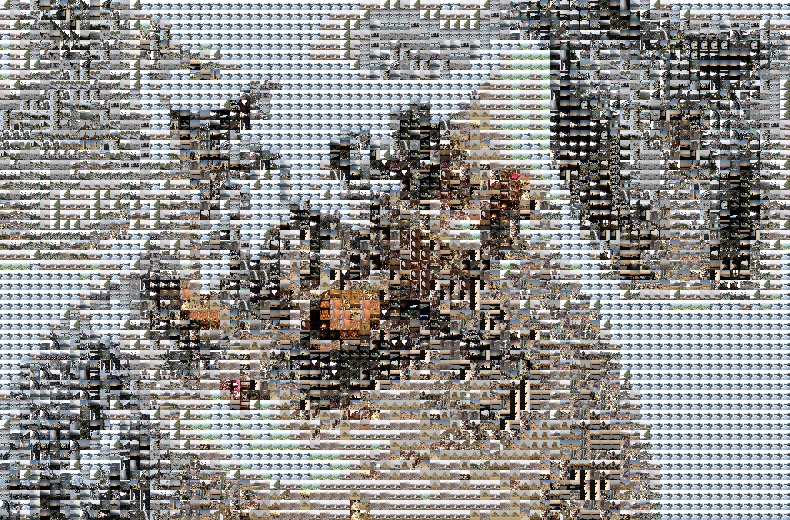
\includegraphics[width=.35\textwidth]{cat-rgb-10.jpg}
%
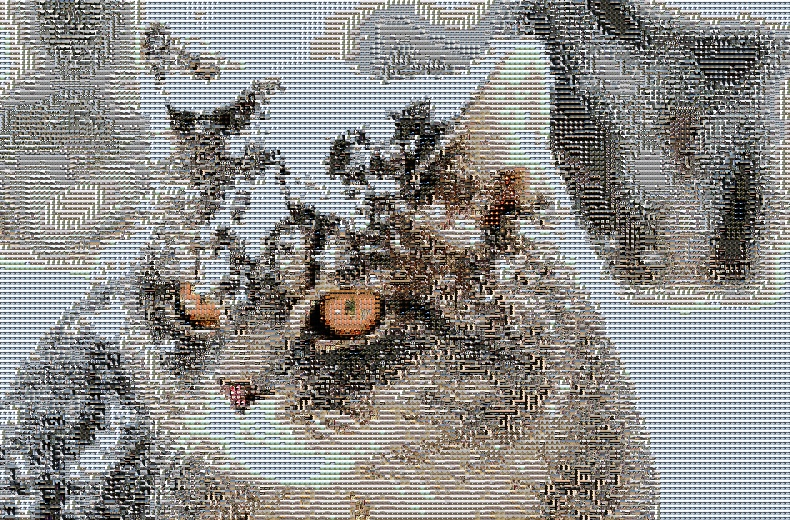
\includegraphics[width=.35\textwidth]{cat-rgb-5.jpg}

\textbf{HSV}\\

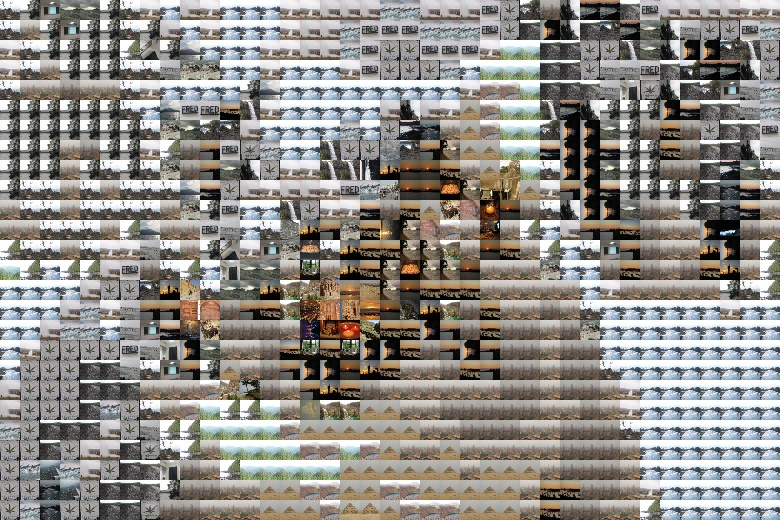
\includegraphics[width=.35\textwidth]{cat-hsv-20.jpg}
%
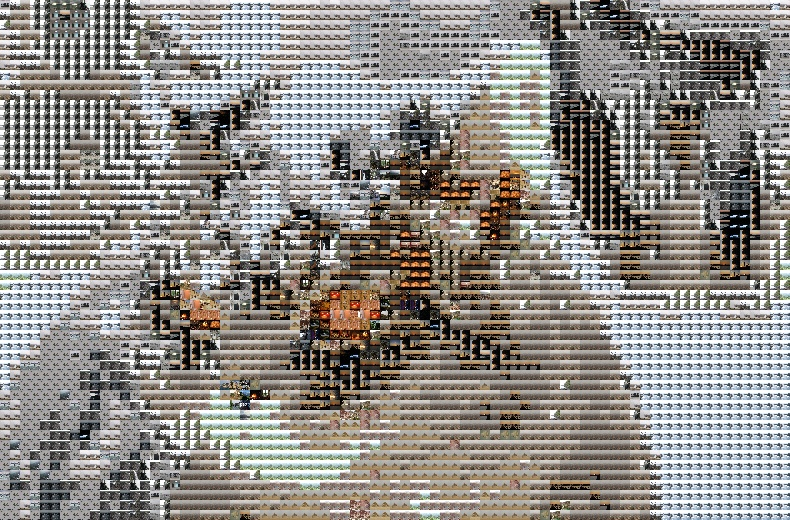
\includegraphics[width=.35\textwidth]{cat-hsv-10.jpg}
%
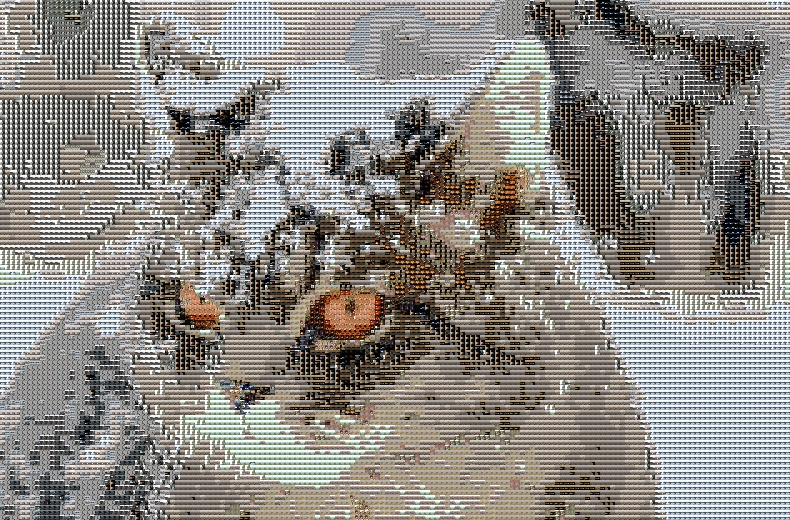
\includegraphics[width=.35\textwidth]{cat-hsv-5.jpg}
\end{frame}

\begin{frame}
\frametitle{Results}
\textbf{Input}\\

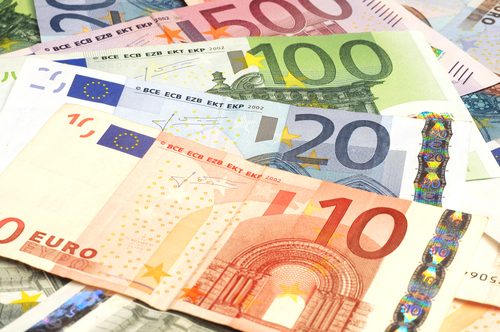
\includegraphics[width=.3\textwidth]{euros.jpg}

\textbf{RGB}\\

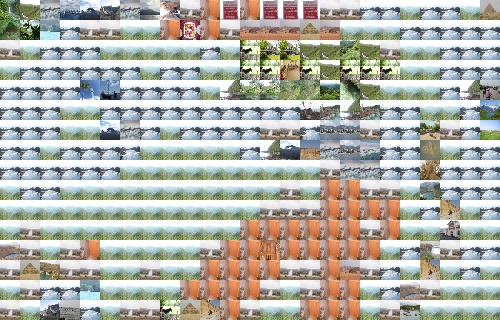
\includegraphics[width=.35\textwidth]{euros-rgb-20.jpg}
%
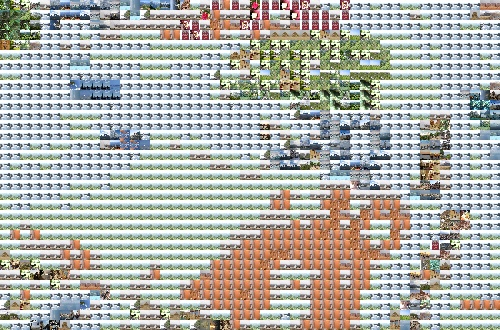
\includegraphics[width=.35\textwidth]{euros-rgb-10.jpg}
%

\includegraphics[width=.35\textwidth]{euros-rgb-5.jpg}
\end{frame}

\begin{frame}
\frametitle{Results}
\textbf{RGB}\\

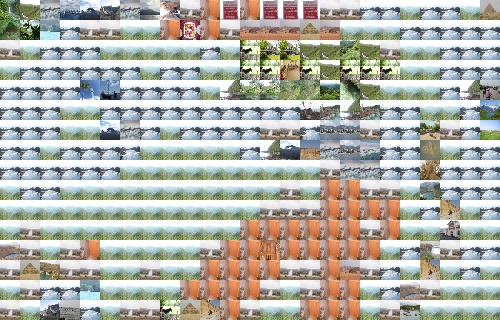
\includegraphics[width=.35\textwidth]{euros-rgb-20.jpg}
%
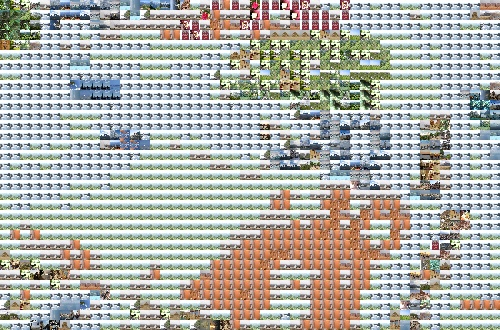
\includegraphics[width=.35\textwidth]{euros-rgb-10.jpg}
%

\includegraphics[width=.35\textwidth]{euros-rgb-5.jpg}

\textbf{HSV}\\

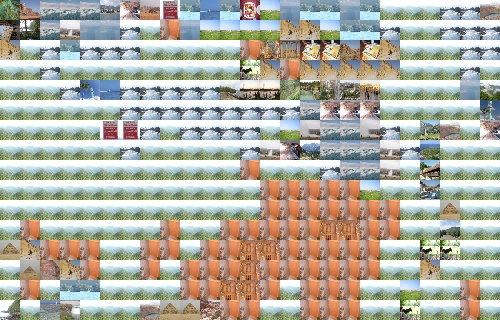
\includegraphics[width=.35\textwidth]{euros-hsv-20.jpg}
%
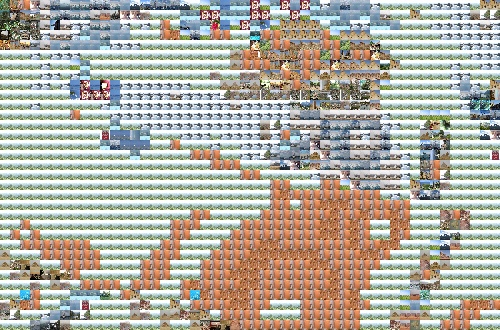
\includegraphics[width=.35\textwidth]{euros-hsv-10.jpg}
%
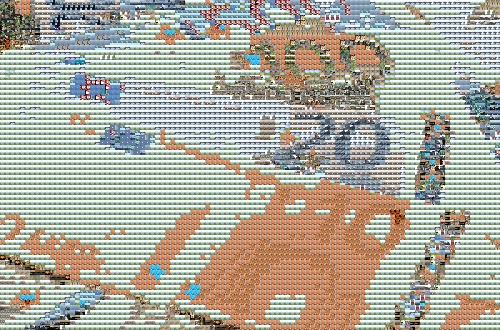
\includegraphics[width=.35\textwidth]{euros-hsv-5.jpg}
\end{frame}


\begin{frame}
\frametitle{Thank you!}

\begin{center}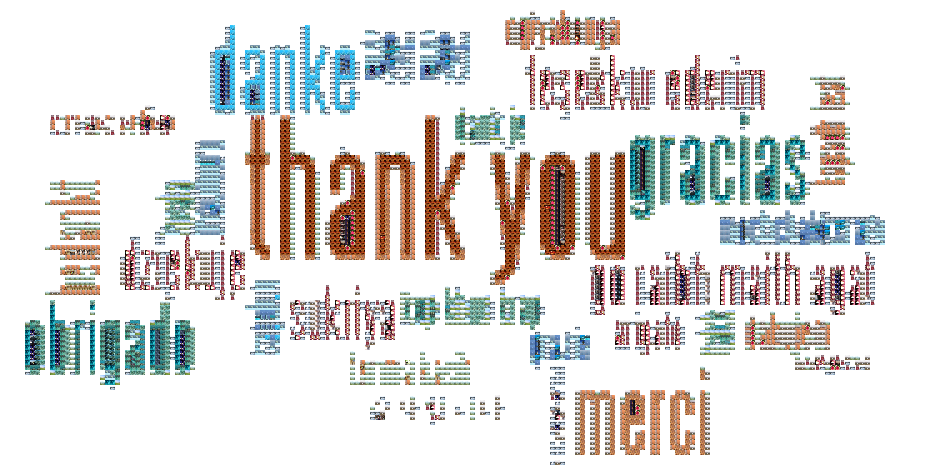
\includegraphics[width=\textwidth]{thank-you5.png}\end{center}

\end{frame}

\end{document}